\section{Results} \label{sec:results}
In this section all the results are collected, where we first determine the energy in the one-dimensional Ising model, and the find the phase. We use linear regression and neural networks, and logistic regression and neural networks respectively for the two cases.

\subsection{Determine the energy in the Ising model}
We have determined the energy of the Ising model using both linear regression (OLS, Ridge and Lasso) and neural networks, where we first train the model on a set, and then validate the model on a test set. In project 1, we found our implementation of OLS, Ridge and Lasso to give the same result as Scikit Learn, and we will in this project stick to Scikit Learn due to its quickness. [1] Let's start with linear regression. 

\subsubsection{Linear regression}
We used linear regression to find the $\bb{J}$-matrix, and from that we found the energies. In table \eqref{tab:lin_reg}, the errors between obtained energy and true energy are listed for the training set, the test set and the K-fold cross-validation resampling. Further, the $\bb{J}$-matrix is visualized in figure \eqref{fig:J_matrix} and the R$^2$-score is plotted as function of $\lambda$ in figure \eqref{fig:lambda_vs_R2_linear}.

\begin{table} [H]
	\caption{Mean Square Error and R$^2$-score presented for OLS, Ridge and Lasso on the Ising model. 'Train' means the results obtained from the training set, containing 8000 states, and 'Test' means the results obtained from the test set, containing 2000 states. The 'K-fold'-columns are results from K-fold resampling with 10 folds. For Ridge and Lasso, we used $\lambda=1e-3$ (penalty). See text for more information.}
	\begin{tabularx}{\textwidth}{l|XXX|XXX} \hline\hline
		\label{tab:lin_reg}
		& \multicolumn{3}{c}{\textbf{MSE}}&\multicolumn{3}{c}{\textbf{R2}}\\ \hline
		&Train&Test&K-fold&Train&Test&K-fold\\ \hline
		OLS & 0.3006 & 0.3006 & 0.3739 & 0.9925 & 0.9927 & 0.9906\\
		Ridge & 1.731e-13 & 2.150-13 & 1.618e-13 & 1.000 & 1.000 & 1.000 \\
		Lasso & 4.029e-5 & 4.189e-5 & 4.0346e-5 & 1.000 & 1.000 & 1.000 \\ \hline\hline
	\end{tabularx}
\end{table}

We observe that the MSE is quite low, especially for Ridge and Lasso. The R$^2$-score is correspondingly high. Below, in figure \eqref{fig:J_matrix}, the $\bb{J}$-matrix is visualized for all the linear regression methods and $\lambda\in[1e-1,1e-6]$.

\newgeometry{left=2cm,right=2cm,top=2cm}
\begin{figure} [H]%
	\centering
	\subfloat[OLS, $\lambda=0.1$]{{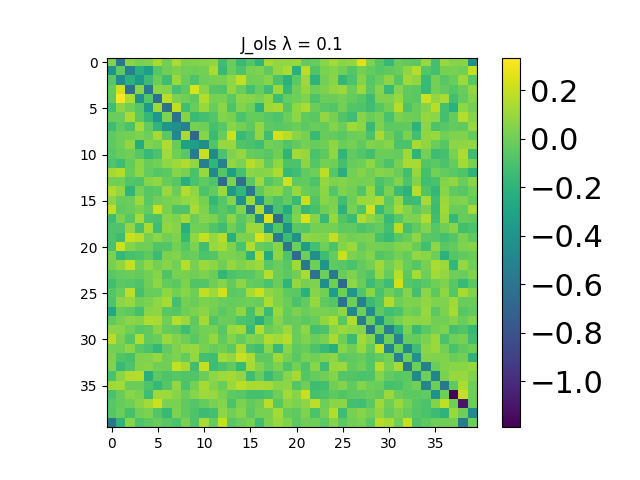
\includegraphics[width=6cm]{../plots/J_ols_lambda_1.png}}}
	\subfloat[Ridge, $\lambda=0.1$]{{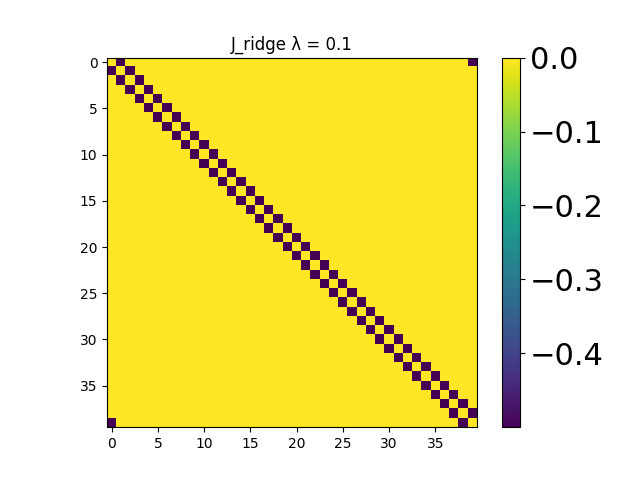
\includegraphics[width=6cm]{../plots/J_ridge_lambda_1.png} }}
	\subfloat[Lasso, $\lambda=0.1$]{{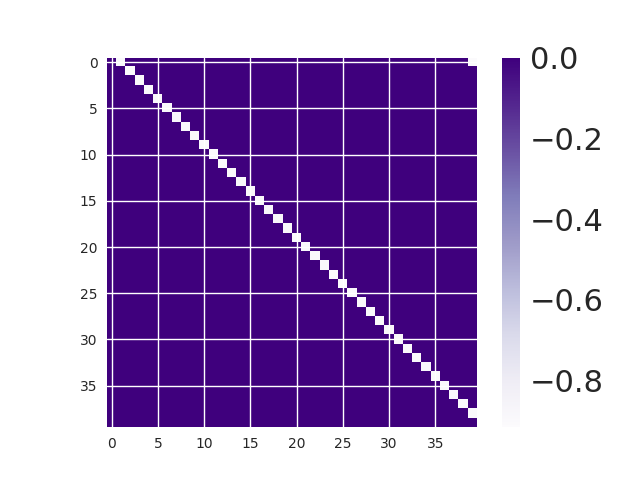
\includegraphics[width=6cm]{../plots/J_lasso_lambda_1.png} }}\\
	
	\subfloat[OLS, $\lambda=0.001$]{{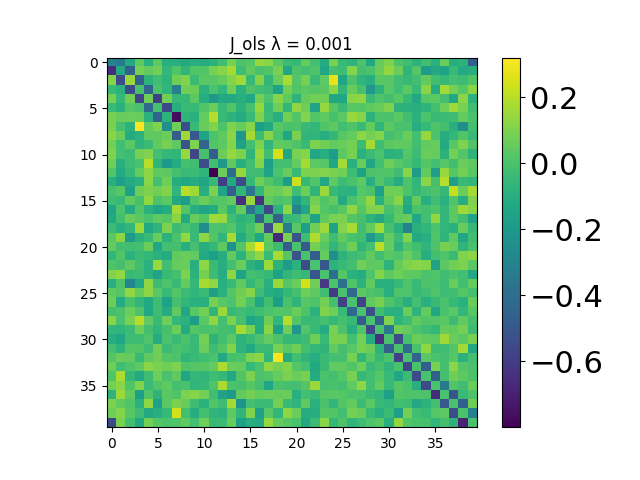
\includegraphics[width=6cm]{../plots/J_ols_lambda_3.png} }}%
	\subfloat[Ridge, $\lambda=0.001$]{{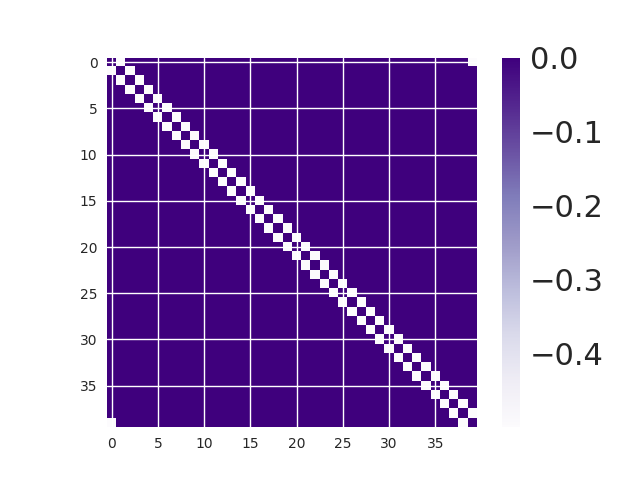
\includegraphics[width=6cm]{../plots/J_ridge_lambda_3.png} }}
	\subfloat[Lasso, $\lambda=0.001$]{{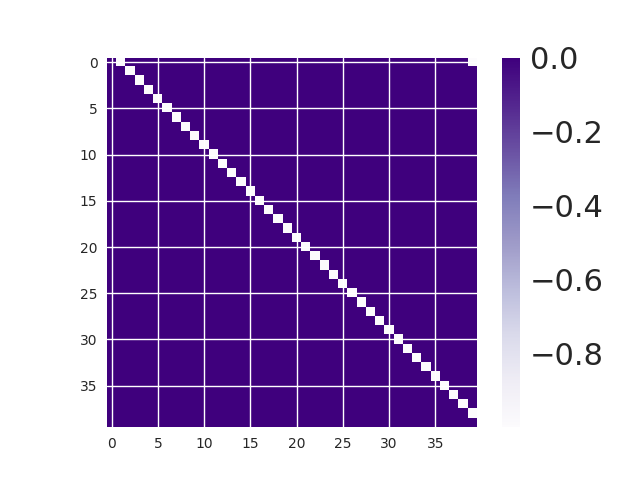
\includegraphics[width=6cm]{../plots/J_lasso_lambda_3.png} }}\\
	
	\subfloat[OLS, $\lambda=0.0001$]{{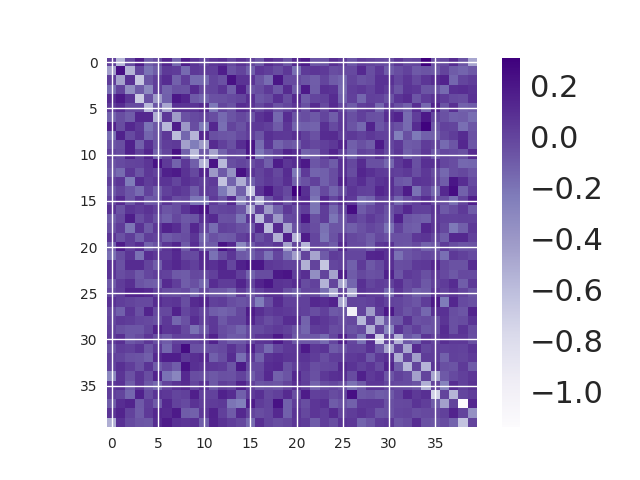
\includegraphics[width=6cm]{../plots/J_ols_lambda_4.png} }}%
	\subfloat[Ridge, $\lambda=0.0001$]{{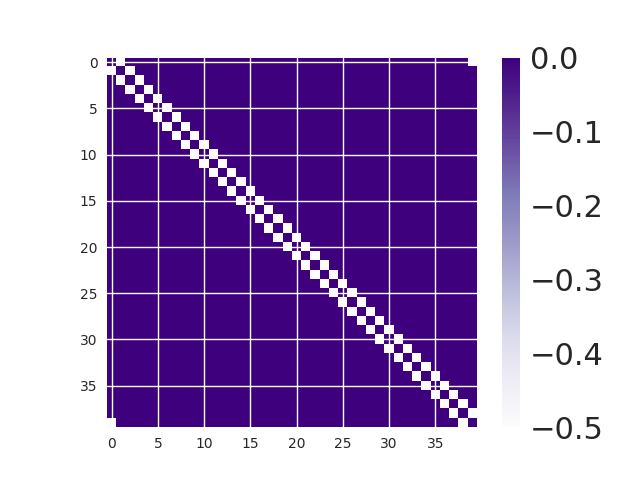
\includegraphics[width=6cm]{../plots/J_ridge_lambda_4.png} }}
	\subfloat[Lasso, $\lambda=0.0001$]{{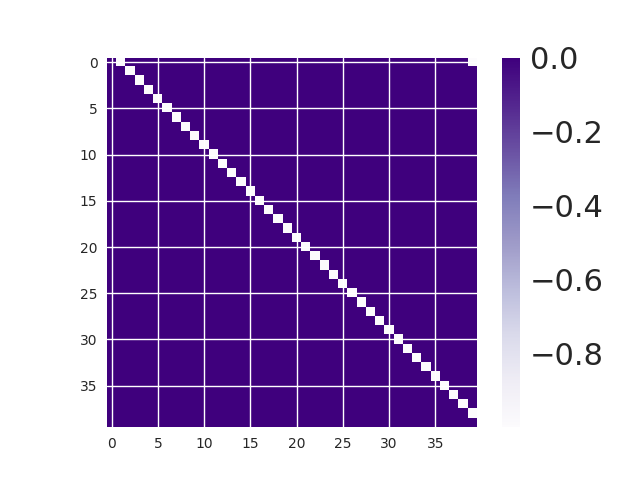
\includegraphics[width=6cm]{../plots/J_lasso_lambda_4.png} }}\\
	
	\subfloat[OLS, $\lambda=0.000001$]{{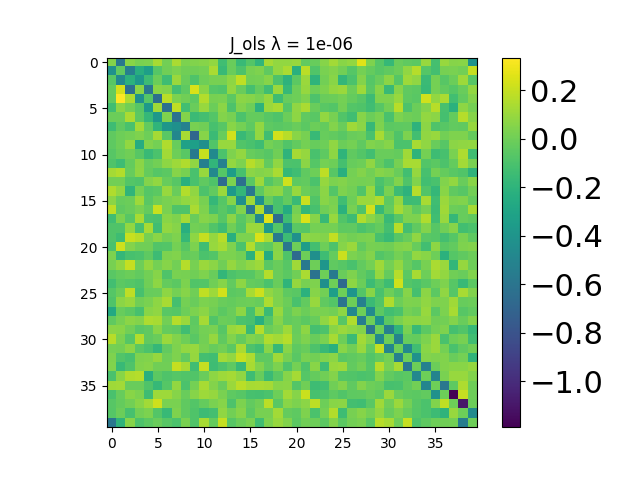
\includegraphics[width=6cm]{../plots/J_ols_lambda_6.png} }}%
	\subfloat[Ridge, $\lambda=0.000001$]{{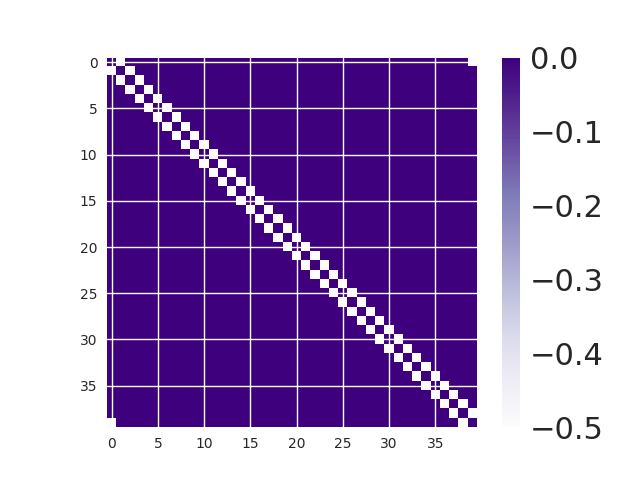
\includegraphics[width=6cm]{../plots/J_ridge_lambda_6.png} }}
	\subfloat[Lasso, $\lambda=0.000001$]{{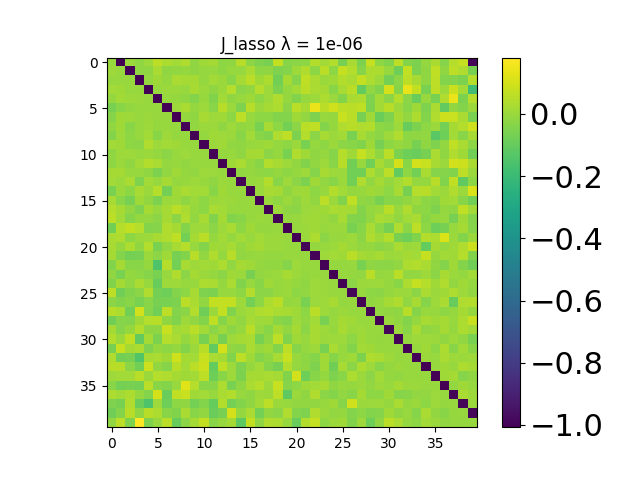
\includegraphics[width=6cm]{../plots/J_lasso_lambda_6.png} }}
	\caption{The J-matrix obtained from OLS, Ridge and Lasso with $\lambda\in[1e-1,1e-6]$. The models where trained on 8000 randomly chosen Ising states.}%
	\label{fig:J_matrix}
\end{figure}
\restoregeometry
We observe that the $\bb{J}$ obtained form Lasso is superdiagonal, while for Ridge it is sub-superdiagonal. For OLS, the matrix tends to be sub-superdiagonal, but the off-diagonal elements are not fully zero. 

Finally, the R$^2$-score is plotted as a function of the penalty, $\lambda$, in figure \eqref{fig:lambda_vs_R2_linear}.
\begin{figure} [H]
	\centering
	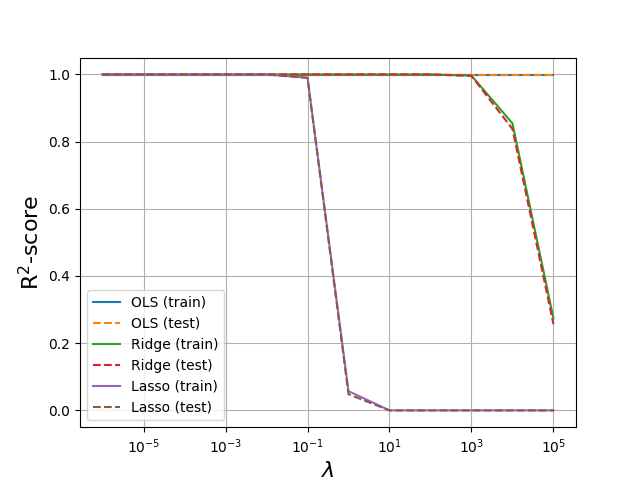
\includegraphics[scale=0.65]{../plots/lambda_vs_R2_linear.png}
	\caption{The R$^2$-score as a function of the penalty. }
	\label{fig:lambda_vs_R2_linear}
\end{figure} 

\subsubsection{Neural networks}
We now want to train a neural network on different Ising states, with the energies as the targets. In table \eqref{tab:nn}, the MSE and R$^2$-score are given for various activation functions in the hidden layer and various number of hidden nodes for the training set, test set and using K-fold cross validation. By far the lowest MSE is obtained when using the pure linear cost function in the hidden layer, and apparently the more nodes the lower MSE. This does not apply for the other activation functions. 
\begin{table} [H]
	\caption{Mean Square Error and R$^2$-score obtained using a neural network on the training set, test set and from K-fold cross validation with $K=10$. Various activation functions \textit{Pure linear}, \textit{ReLU}, \textit{Leaky ReLU} and \textit{ELU} were used in the hidden layer, and the number of hidden nodes, H, was set to 0, 5 and 10. The learning rate was set to $\eta=0.0001$ and we used $T=5$ minimization iteration in GD.}
	\begin{tabularx}{\textwidth}{l|l|XXX|XXX} \hline\hline
		\label{tab:nn}
		&& \multicolumn{3}{c}{\textbf{MSE}}&\multicolumn{3}{c}{\textbf{R2}}\\ \hline
		&H&Train&Test&K-fold&Train&Test&K-fold\\ \hline
		
		\parbox[t]{2mm}{\multirow{3}{*}{\rotatebox[origin=c]{90}{Linear}}}
		&0 & 3.244e-4 & 5.573e-4 & 1.206e-4 & 1.000 & 1.000 & 1.000\\
		&5 & 1.545e-9 & 2.690e-9 & 2.375e-3 & 1.000 & 1.000 & 1.000 \\
		&10 & 6.905e-11 & 7.848e-11 & 3.932e-10 & 1.000 & 1.000 & 1.000\\ \hline
		
		\parbox[t]{2mm}{\multirow{3}{*}{\rotatebox[origin=c]{90}{ReLU}}}
		&0 & 3.196e-4 & 5.511e-4 & 1.188e-4 & 1.000 & 1.000 & 1.000 \\
		&5 & 8.618e-1 & 1.107e-0 & 2.405e-1 & 0.9779 & 0.9712 & 0.9939 \\
		&10 & 1.600e-1 & 1.797e-1 & 1.994e-1 & 0.9959 & 0.9953 & 0.9943\\ \hline
		
		\parbox[t]{2mm}{\multirow{3}{*}{\rotatebox[origin=c]{90}{Leaky}}}
		&0 & 3.182e-4 & 5.481e-4 & 1.174e-4 & 1.000 & 1.000 & 1.000 \\
		&5 & 4.128e-1 & 4.627e-1 & 2.230e-1 & 0.9894 & 0.9880 & 0.9943\\
		&10 & 1.965e-1 & 2.115e-1 & 2.394e-1 & 0.9949 & 0.9945 & 0.9939\\ \hline
		
		\parbox[t]{2mm}{\multirow{3}{*}{\rotatebox[origin=c]{90}{ELU}}}
		&0 & 3.449e-4 & 6.472e-4 & 1.198e-4 & 1.000 & 1.000 & 1.000\\
		&5 & 2.414e-1 & 2.546e-1 & 1.463e-1 & 0.9405 & 0.9342 & 0.9535\\
		&10 & 1.223e-1 & 2.281e-1 & 5.359e-1 & 0.9970 & 0.9941 & 0.9862\\ \hline\hline
	\end{tabularx}
\end{table}


\subsection{Classifying the phase}
We now turn to the classification problem, where we want to find whether an Ising lattice is ordered or disordered. We exclude Ising lattices around critical temperature in our training set ("Train", 100000 states), and test our model on unseen data ("Test", 30000 states). Additionally, we also test our model on lattices which are close to the critical temperature ("Critical", 30000 states).  We first use logistic regression with logistic activation, and thereafter turn to neural network with various activation functions on the hidden layer and logistic activation on the output. 

\subsubsection{Logistic regression}
Our first approach is the logistic regression. For this, we calculate the accuracy for various learning rates and regularizations, given in figure \eqref{fig:class_logistic} for all three data sets. What we observe, is that the model is really sensitive and the accuracy vary a lot. For some specific learning rates and regularization parameters, we get good result even for the critical set.
\newgeometry{left=2cm,right=2cm,top=1.5cm}
\begin{figure} [H]%
	\centering
	\subfloat[Train]{{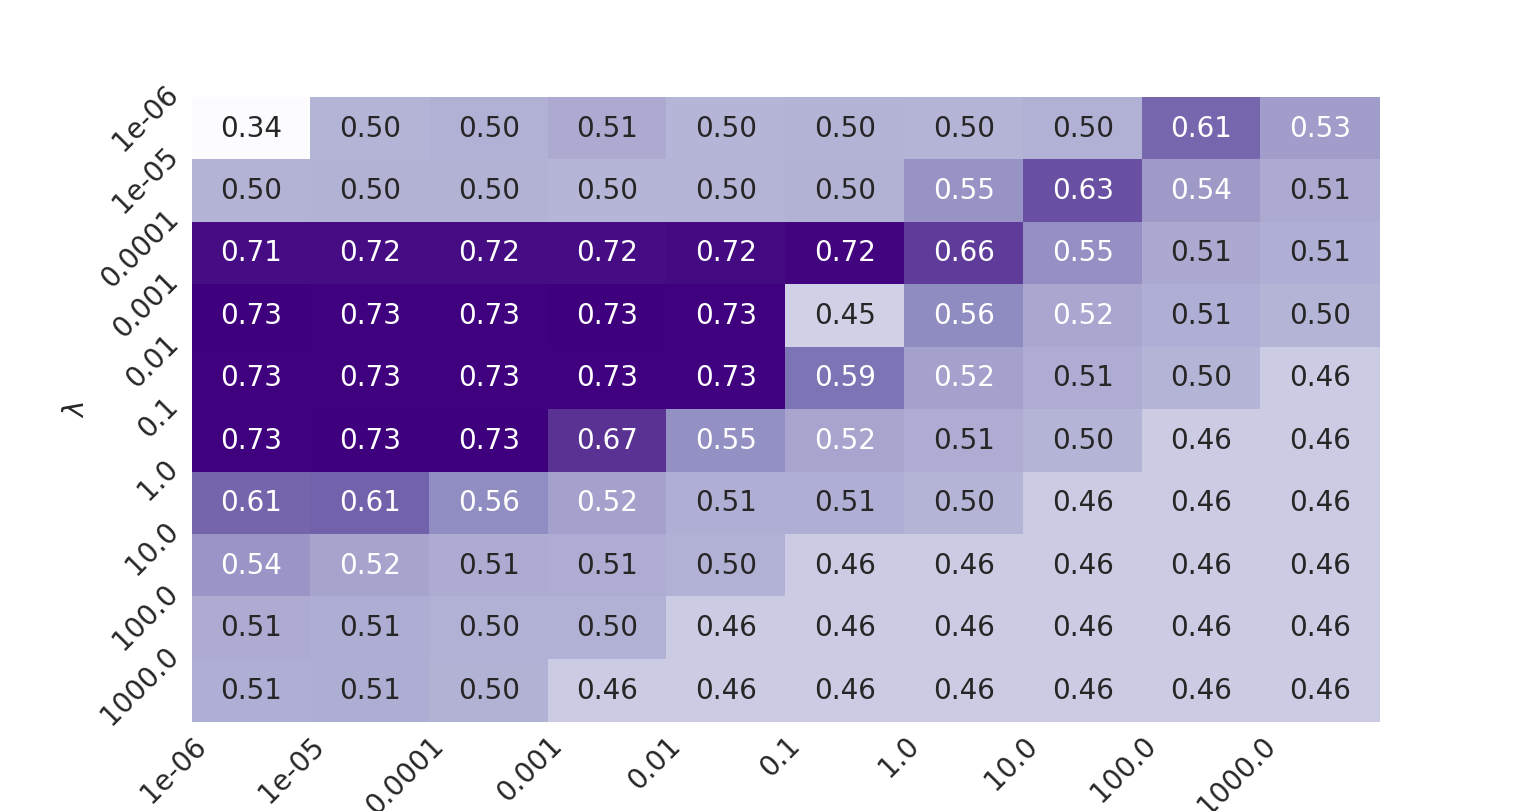
\includegraphics[width=13cm]{../plots/classification_logistic_train.png}}}\\
	
	\subfloat[Test]{{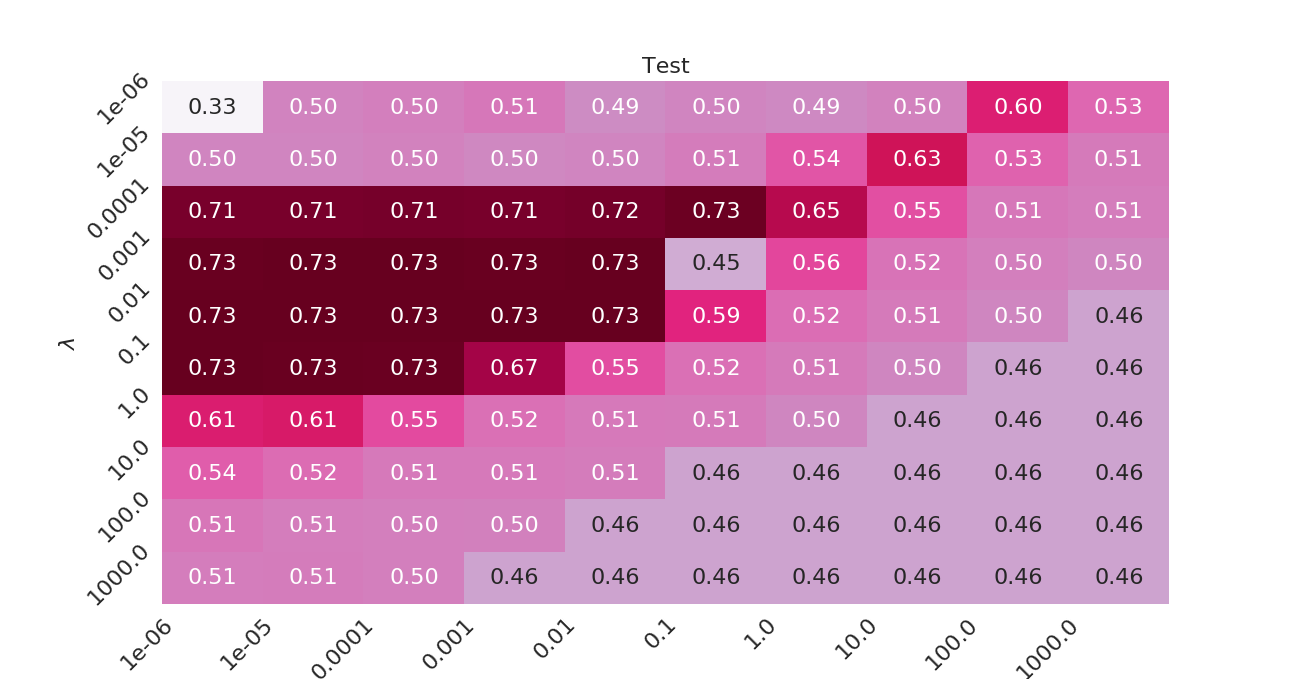
\includegraphics[width=13cm]{../plots/classification_logistic_test.png} }}\\
	
	\subfloat[Critical]{{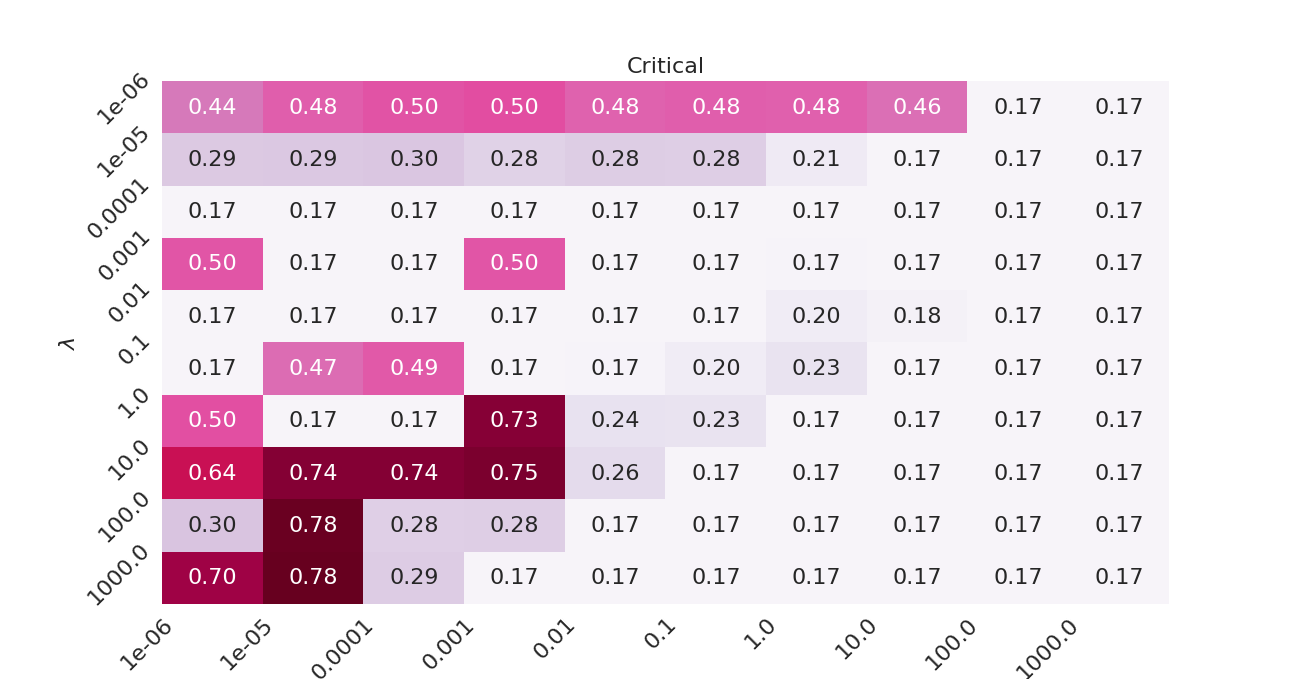
\includegraphics[width=13cm]{../plots/classification_logistic_critical.png} }}\\
	
	\caption{The accuracy score as function of the learning rate $\eta\in[1e-6,1e3]$ and regularization parameter $\lambda\in[1e-6,1e3]$ for the training set (a), test set (b) and critical set (c).}%
	\label{fig:class_logistic}
\end{figure}
\restoregeometry

\subsubsection{Neural networks}
Our second and final approach is classification using neural network. In the same way as when we used neural network in regression, we will investigate various activation functions in the hidden layer(s). 
\begin{table} [H]
	\caption{The accuracy obtained using neural network for classification. 'Train' is the training set, 'Test' is a test set far from critical temperature and 'Critical' is a test set close to the critical temperature. We used one minimization iteration ($T=1$), learning rate $\eta=1e-4$ and regularization parameter $\lambda=1e-3$, used logistic activation function on output node and tried \textit{pure linear}, \textit{ReLU} and \textit{Leaky ReLU} on the hidden layers. Notation "10+10" means two layers of 10 hidden nodes each.}
	\begin{tabularx}{\textwidth}{l|l|XXX} \hline\hline
		\label{tab:nn_class}
		&& \multicolumn{3}{c}{\textbf{Accuracy}}\\ \hline
		&Hidden nodes&Train&Test&Critical\\ \hline
		
		\parbox[t]{2mm}{\multirow{3}{*}{\rotatebox[origin=c]{90}{Linear}}}
		&10 & 0.4371 & 0.4381 & 0.3333 \\
		&10+10 & 0.4379 & 0.4367 & 0.3333 \\
		&10+10+10 & 0.4371 & 0.4382 & 0.3333 \\ \hline
		
		\parbox[t]{2mm}{\multirow{3}{*}{\rotatebox[origin=c]{90}{ReLU}}}
		&10 & 0.9930 & 0.9929 & 0.9655 \\
		&10+10 & 0.9935 & 0.9934 & 0.9679 \\
		&10+10+10 & 0.9935 & \textbf{0.9938} & \textbf{0.9686} \\ \hline
		
		\parbox[t]{2mm}{\multirow{3}{*}{\rotatebox[origin=c]{90}{Leaky}}}
		&10 & 0.9931 & 0.9929 & 0.9656 \\
		&10+10 & 0.9932 & 0.9933 & 0.9668 \\
		&10+10+10 & \textbf{0.9936} & 0.9935 & 0.9685 \\ \hline\hline
	\end{tabularx}
\end{table}

\begin{figure} [H]
	\centering
	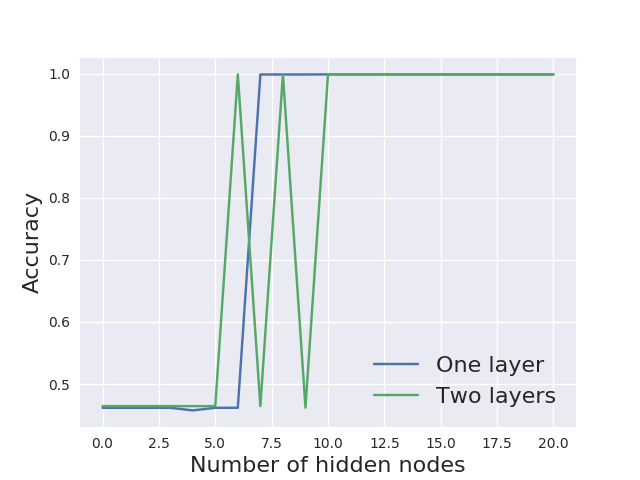
\includegraphics[scale=0.45]{../plots/h_vs_accuracy.png}
	\caption{Accuracy as a function of number of hidden nodes, for both one and two layers. X-axis indicates number of hidden nodes in each layer, where the two-layer perceptron has an equal number of nodes in each layer.}
	\label{fig:h_vs_accuracy}
\end{figure} 
